%!TEX root = ../report.tex

% 
% Related work
% 

\section{Related Work}

% Example citation:
In this section we will present a set of literature references on the subjects related to this thesis. We will present the most important frameworks on Information Systems Management and Governance. This process has the objective to come up with a choice of a frameworks or a set of them to implement our processes for project and maintenance management.\par
In terms of logical application architectures, we will provide an analysis of the main features of a set of Project Management and IT Service Management solutions available on the market. Our objective is to conduct a comparative analysis relating all the solutions and choose the ones that best fit our purposes for use on an logical application architecture.  

\subsection{Frameworks for Information Technologies Governance and Management}

In this section we will present the three frameworks we consider the most relevant for this thesis: COBIT 5, ITIL V3 and PMBOK. This three frameworks provide, from different perspectives, guides and principles for IT Governance and Management, providing processes for achieving a successful implementation of this principles in an organization.\par


\subsubsection{IT Governance and IT Management}

One important concept to define is the difference between IT Governance and IT management. They are many times confused and some authors already tried to explain the difference between the two concepts.\par
Considering the definition given by Van Grembergen \textit{et al.}, ``''IT Management is focused on the internal effective supply of IT services and products and the management of present IT operations. IT Governance in turn is much broader, and concentrates on performing and transforming IT to meet present and future demands of the business (internal focus) and the business' customers (external focus).``''.\par
 Considering the COBIT 5 view for this question, it makes a clear distinction between governance and management, in the way these two disciplines encompass different types of activities, require different organizational structures and serve different purposes. Governance ensures that stakeholders' needs, conditions and options are evaluated to determine balanced, agreed-on enterprise objectives to be achieved. it sets direction through prioritisation and decision making and monitors performance and compliance against agreed-on direction and objectives.On the other hand, management plans, builds, runs and monitors activities in alignment with the direction set by the governance body to achieve the enterprise objectives.\par

\begin{figure}
\centering
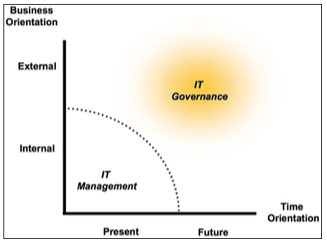
\includegraphics[width=0.6\textwidth]{img/ITGovernanceAndManagement.png}
\caption{IT Governance and IT Management}
\end{figure}


 Considering both definitions and the figure 1, we can conclude that IT Governance has a bigger dimension that IT Management, but both need to be related and complementary to achieve success inside an organization. It is not possible for an organization to have well defined and matured management processes that are no related to governance aspects, but governance needs management to achieve goals and objectives settled to achieve success.

\subsubsection{COBIT 5}

Control Objectives for Information and Related Technology (COBIT) is a framework created by the Information Systems Audit and Control Association (ISACA) for IT Management and IT Governance.\par
COBIT 5 provides a comprehensive framework that assists enterprises in achieving their objectives for the governance and management of enterprise IT. Simply stated, it helps enterprises create optimal value from IT by maintaining a balance between realizing benefits and optimizing risk levels and resource use \cite{2012cobit}. The framework is built on five basic principles:

\begin{itemize}
  \item Meeting the Stakeholders Needs 
  \item Covering the Enterprise End-to-end
  \item Applying a Single, Integrated Framework
  \item Enabling a Holistic Approach
  \item Separating Governance from Management
\end{itemize}


It also defines seven enablers, explained by COBIT as factors that, individually and collectively, influence whether governance and management over enterprise will work or not. This enablers can be categorized as:

\begin{itemize}
  \item Principles, Policies and frameworks 
  \item Processes 
  \item Organizational structures
  \item Culture, ethics and behavior 
  \item Information
  \item Services, infrastructure and applications
  \item People, skills and competencies
\end{itemize}

\begin{figure}
\centering
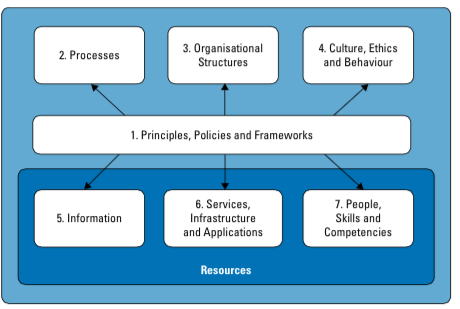
\includegraphics[width=0.7\textwidth]{img/Enablers.png}
\caption{COBIT 5 enablers}
\end{figure}

Figure 2 presents the COBIT 5 enablers previous defined and how they relate among themselves int terms of its importance for organization. Each enabler has stakeholders, a set of goals, a life cycle and can be defined good practices for each one.\par

\begin{figure}
\centering
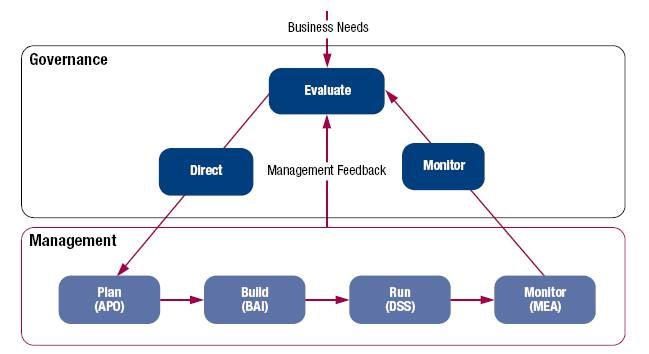
\includegraphics[width=0.9\textwidth]{img/COBITProcesses.jpg}
\caption{COBIT 5 domains}
\end{figure}

Considering figure 3, COBIT 5 process reference model considers two big domains of processes: Governance and Management. The governance domain contains five processes in the domain Evaluate, Direct and Monitor(EDM). The management domain has four internal domains of processes: Align, Plan and Organise(APO), Build, Acquire and Implement(BAI), Deliver, Service and Support (DSS) and Monitor, Evaluate and Assess(MEA).\par
All processes for management and governance are presented in the appendix and all the implementation details explained in COBIT 5: Enabling Processes, A detailed reference guide to the processes defined in the COBIT 5 process reference model. This includes the COBIT 5 goals cascade, a process model explanation, governance and management practices, and the process reference model\cite{2012cobitEP}.\par
COBIT 5 includes a process capability model based on ISO/IEC 15504 Software Engineering - Process Assessment standard. [REFERENCE HERE] This model allow to measure the current level of maturity of enterprise processes, presenting the gap between the current level and the desired one the enterprise wants to achieve. This new capability model is an improvement of the previous on COBIT 4.1, being more simplified and compliant with a generally accepted process assessment standard.\par
Relating to other frameworks and standards, COBIT tries to establish a framework that is compliant with the most widely accepted standards in IT governance and management. In figure 4 we can see the standards COBIT 5 relates by processes domain, with special attention to ITIL V3, ISO/IEC 20000, PMBOK and CMMI, that are closely related to this thesis problem. This compliance with other standards is fundamental for a widely adoption of COBIT 5, in the way it tries to establish goals, metrics, practices, roles, inputs and outputs for each process, making it necessary being compliant with international standards. This will improve COBIT application and acceptance on organizations.\par

\subsubsection{COBIT 5 critical analysis}

The COBIT 5 is one of the most interesting frameworks widely accepted by organizations in the IT management and Governance area. It arises as the main framework for establishing processes to guide us on management and governance and establish ways to control them. However, it is a complex framework that needs time and practice to be fully implemented.\par
For this thesis project, we will consider only the domains relevant for our objectives, making a selection of the processes we pretend to implement. This will allow us to get the bigger value COBIT has to offer, making it possible, in the time-frame available, achieve our implementation objectives.\par
One important aspect of the use of COBIT is that it provides a more business and strategic view of IT on organizations, presenting a lack of operational approach to some themes that are relevant for our project. To overcome this, we will analyze a more operational framework on IT service management, the ITIL V3 framework\cite{itilIntro,itilSS,itilST,itilSD,itilSO,itilCSI} and a project management guide considered by the main specialists on the area as the reference for project management, the Project Management Book of Knowledge\cite{pmbok5}.\par

\begin{figure}
\centering
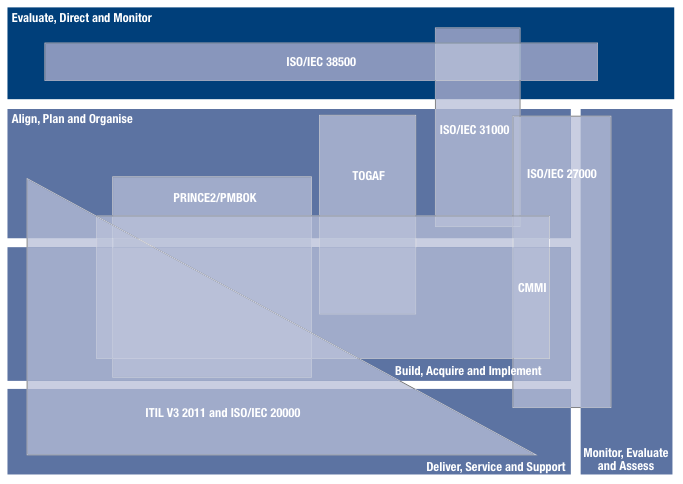
\includegraphics[width=0.9\textwidth]{img/COBITOtherFrameworks.png}
\caption{COBIT 5 coverage on other frameworks}
\end{figure}

\subsubsection{ITIL V3}

First developed in the 1980s by the actual Office of Government Commerce (OGC), a branch of the British Government, ITIL defines processes for IT Service management at a high level, being left to the organizations to implement the processes in the manner most suitable to their particular situations and needs.\par
ITIL is becoming a de facto standard worldwide as organizations adopt it as their guideline for establishing IT service management (ITSM) processes. IT organizations can use the guidance provided by ITIL to transform their service management capabilities into strategic assets, those that provide the basis for core competence, distinctive performance, durable advantage, and qualifications to participate in business opportunities.\par
The ITIL service management practices are comprised of three main sets of products and services: ITIL service management practices (core guidance), ITIL service management practices (guidance specific to industry sectors, organization types, operating models and technology architectures) and ITIL web support services.\par

\begin{figure}
\centering
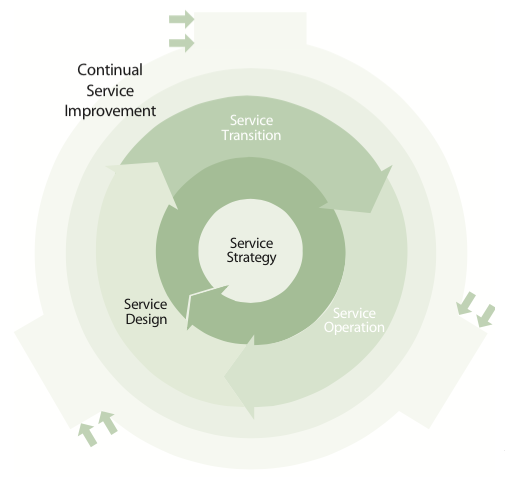
\includegraphics[width=0.7\textwidth]{img/ITILVolumes.png}
\caption{ITIL V3 volumes}
\end{figure}

The core set, presented in figure 5 and the one we will consider for this thesis, consists of six publications: Introduction to ITIL Service Management Practices, Service Strategy, Service Design, Service Transition, Service Operation and Continual Service Improvement. Each one of this volumes share the same conceptual structure, being composed by practice fundamentals and principles, life cycle processes and activities, supporting organization structures and roles, technology considerations, practice implementation and challenges, risks and critical success factors.

\paragraph{\textbf{Service Strategy}} provides guidance on how to view service management not only as an organizational capability but as a strategic asset. Guidance is provided on the principles underpinning the practice of service management which are useful for developing service management policies, guidelines and processes across the ITIL Service Lifecycle.\cite{itilSS} The processes included in Service Strategy volume are:

\begin{itemize}
  \item Financial Management
  \item Service Portfolio Management 
  \item Demand Management
\end{itemize}

\paragraph{\textbf{Service Design}} provides guidance for the design and development of services and service management practices. It covers design principles and methods for converting strategic objectives into portfolios of services and service assets. The scope of Service Design is not limited to new services. It includes the changes and improvements necessary to increase or maintain value to customers over the life cycle of services, the continuity of services, achievement of service levels, and conformance to standards and regulations.\cite{itilSD} The processes included in Service Design volume are:

\begin{itemize}
  \item Service Catalogue Management
  \item Service Level Management 
  \item Capacity Management
  \item Availability Management
  \item IT service Continuity Management
  \item Information Security Management 
  \item Supplier Management
  \item Application Management
  \item Data and Information Management
  \item Business Service Management
\end{itemize} 

\paragraph{\textbf{Service Transition}} provides guidance for the development and improvement of capabilities for transitioning new and changed services into live service operation. This publication provides guidance on how the requirements of Service Strategy encoded in Service Design are effectively realized in Service Operation while controlling the risks of failure and disruption.\cite{itilST} The processes included in Service Transition volume are:

\begin{itemize}
  \item Change Management
  \item Service asset and Configuration Management
  \item Release and deployment Management
  \item Knowledge Management
  \item Stakeholder Management
  \item Transition Planning 
  \item Support and Service Evaluation 
\end{itemize} 

\paragraph{\textbf{Service Operation}} embodies practices in the management of the day-to-day operation of services. It includes guidance on achieving effectiveness and efficiency in the delivery and support of services to ensure value for the customer and the service provider. Strategic objectives are ultimately realized through Service Operation, therefore making it a critical capability. Guidance is provided on how to maintain stability in service operations, allowing for changes in design, scale, scope and service levels.\cite{itilSO} The processes included in Service Operation volume are:

\begin{itemize}
  \item Event Management
  \item Incident Management
  \item Request Management
  \item Problem Management
  \item Access management
\end{itemize} 

\paragraph{\textbf{Continual Service Improvement}} provides instrumental guidance in creating and maintaining value for customers through better design, transition and operation of services. It combines principles, practices and methods from quality management, change management and capability improvement. Organizations learn to realize incremental and large-scale improvements in service quality, operational efficiency and business continuity. Guidance is provided for linking improvement efforts and outcomes with service strategy, design and transition.\cite{itilST} The processes included in Continual Service Improvement volume are:

\begin{itemize}
  \item The 7-Step Improving Process
  \item Service Level Management
\end{itemize} 

\par Not different from COBIT,  ITIL takes public frameworks and standards as a form of the organization to have advantage on the market. Organizations should build their proprietary knowledge on top of a body of knowledge based on public frameworks and standards. Collaboration and coordination across organizations are easier because of shared practices and standards. According to a research performed by the UK Department of Trade and Industry (DTI), the value to the UK economy from standards is estimated to be about \textsterling2.5 billion per annum \cite{McNeillis01112005}.\par
For related standards and frameworks to ITIL V3, we have ISO/IEC 20000 (service management system standards), ISO/IEC 27001 (standard providing requirements for an information security management system), PMBOK (manual for a set of standard terminology and guidelines for project management)\cite{pmbok5} and COBIT\cite{2012cobit}, already presented. This are the standards we will cover for our thesis by being directly related to ITIL V3 and its implementation.


\subsubsection{ITIL V3 critical analysis}

One crucial aspect for the importance of ITIL on this thesis is the operational view that it provides for IT Service Management. ITIL tries to focus on more management details, providing a more practical guidance for implementation. It is focused on IT Service Management and presents concrete guidance for managing services during its life cycle. De Haes and Van Grembergen state that COBIT tells what to do and ITIL explains how to do it, what makes COBIT adopting a process-focused approach and ITIL a service level-oriented one \cite{ITGovAndMech}.\par
The main objective to include ITIL knowledge for this thesis is to provide a complementary guidance on IT management, enhancing the business oriented view of COBIT with a operational view. COBIT 5 will allow us to take advantage of this complementarity, related to the concern of ISACA to make it more compliant with other frameworks, including COBIT, on the new version (relating to COBIT 4.1). 

\subsubsection{PMBOK: A Guide to the Project Management Book of Knowledge}

The Guide to the Project Management Body of Knowledge provides guidelines for managing individual projects and defines project management related concepts. It also describes the project management life cycle and its related processes, as well as the project life cycle.\cite{pmbok5}\par
This guide is considered by many professionals in the area of business management as the main reference for processes and good practices in project management, in the way it defines the knowledge that are applicable to most project most of the time, and there is consensus about their value and usefulness.\par 
The processes are presented relating them with the knowledge area they belong. The PMBOK presents the following areas of project management:

\begin{itemize}
  \item Integration Management
  \item Scope Management
  \item Time Management
  \item Cost Management
  \item Quality management
  \item Human resource management
  \item Communications management
  \item Risk management
  \item Procurement management
  \item Stakeholder management
\end{itemize} 

Each group of processes is related with the life cycle of a project, being also grouped in five categories: Initiating, Planing, Executing, Monitoring and Control and Closing, directly related to the phase they are applied on the life cycle. For each process, it is presented the inputs, tools, techniques and outputs that are required to successfully implement it. All processes organized by group and area are presented in figure 6\par

\begin{figure}
\centering
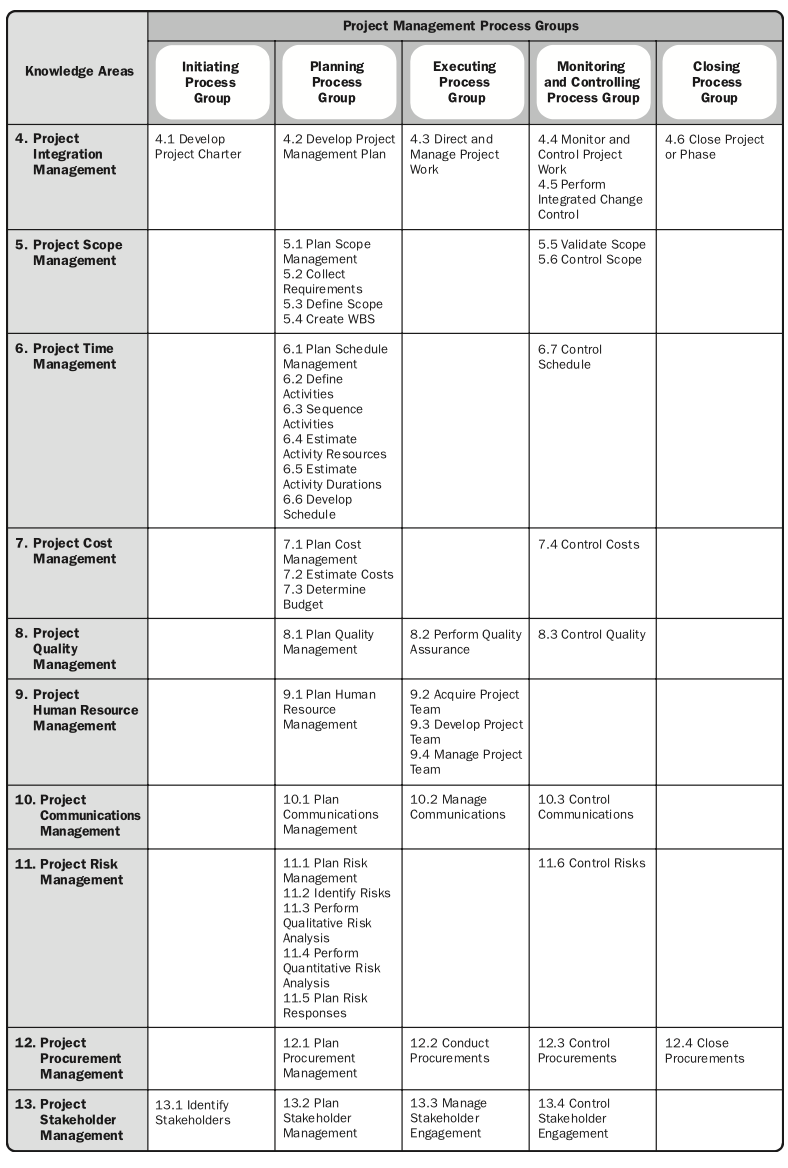
\includegraphics[width=\textwidth]{img/PMBOKprocesses.png}
\caption{PMBOK processes organized by group and area of knowledge}
\end{figure}


This guide also provides some background on the project management area, defining common vocabulary and establishing concepts necessary to fully understand all processes. Presents characteristics of projects, programmes and portfolios, roles of project managers and organizational aspects that influence the management process, like organizational structures, culture, assets or stakeholders.\par 
Another important aspect of PMBOK is that is a more general framework, making it necessary to complement with other frameworks or guides when applying to a specific area. This guide only presents the general processes for project management, lacking on implementation details for specific areas, like the area of IT Management.\par 

\subsubsection{PMBOK critical analysis}

The importance of PMBOK for this thesis is related to its widely acceptance and adoption as the reference guide to project management by many professionals in the area, being tested and evaluated its importance in terms of good practices adopted in project management. Despite being more general and lacking in specificity to IT management, it can be complemented with the two previous frameworks presented (COBIT and ITIL), using some more detailed guidance of ITIL and COBIT to improve PMBOK focus to this thesis.\par
PMBOK presents processes for all phases of the life cycle of a project, being too extensive considering the theme of this thesis and the time-frame available. For this scope, we will only be able to consider a subset of all processes presented, being necessary, in the solution's architecture phase of this thesis, present a mapping between processes covered on PMBOK relating with processes of COBIT and ITIL.


\subsection{International standards}

In this section we will present the international standards that are referenced or important to complement the frameworks previously presented. These standards will allow us to design processes in conformance with practices that are considerer as the reference in some areas of project management.\par
We will analyze the ISO/IEC 12207, an systems and software engineering international standard for Software life cycle processes. This standard will allow us to define the processes that are important to consider in the scope of this thesis. It will provide an high-level process reference for the complete life cycle of a software system\par
Relating to COBIT, we have standards that are directly related to it, as the ISO/IEC 20000, a set of international standards for IT service management, and ISO/IEC 27000, a set of international standards for information security management systems. COBIT also relates with CMMI, the Capability Maturity Model Integration that is a framework for process improvement in business comprising models, appraisal methods, and training.\par
For other standards more general to all frameworks we will present the ISO 31000, a set of standards that provide principles, framework and a process for managing risk, and ISO 19011, a international standard for providing guidelines for auditing management systems. This standards will complement complex areas of project management providing some additional and specific knowledge.

\subsubsection{ISO/IEC 12207}

ISO/IEC 12207:2008 establishes a common framework for software life cycle processes, with well-defined terminology, that can be referenced by the software industry. It contains processes, activities, and tasks that are to be applied during the acquisition of a software product or service and during the supply, development, operation, maintenance and disposal of software products.The purpose of this International Standard is to provide a defined set of processes to facilitate communication among acquirers, suppliers and other stakeholders in the life cycle of a software product.\par
This standard combines the processes to be performed during the life cycle of a software project into seven groups . Each process is described in terms of its objectives and expected results and presents activities to be undertaken to achieve these same objectives. The processes are grouped in 7 groups, related to the phase they are applied during the software life cycle. All processes are listed in figure XXX.

\begin{itemize}
  \item Agreement processes
  \item Organizational Project-Enabling Processes
  \item Project Processes
  \item Technical Processes
  \item Software Implementation Processes
  \item Software Support Processes
  \item Software Reuse Processes 
\end{itemize}

 
\begin{figure}[t!]
\centering
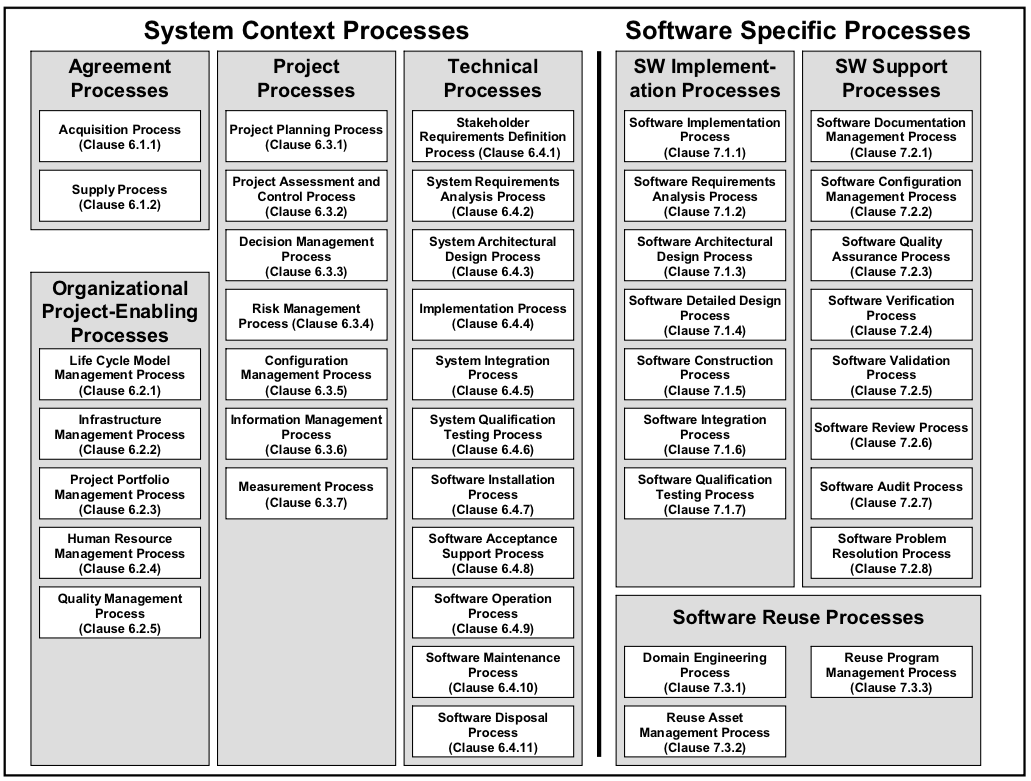
\includegraphics[width=\textwidth]{img/ISO12207Processes.png}
\caption{ISO/IEC 12207 processes}
\end{figure}

This standard may be used standalone or jointly with ISO/IEC 15288, and supplies a process reference model that supports process capability assessment in accordance with ISO/IEC 15504, a set of technical standards documents for the computer software development processes assessment.\par
This standard is important for this thesis in the way it standardize the processes for the whole life cycle of the software, grouping the processes for a better understanding its scope. We will use this standard, specifically figure 7, to present the processes that make part of the scope of this thesis, after what we will relate them with the frameworks previously presented. 


\subsubsection{ISO/IEC 20000}

ISO/IEC 20000 corresponds to a standard on IT Service Management. Initially was developed to reflect best practice guidance contained in some frameworks like ITIL, COBIT or Microsoft operations. This standard in composed by 5 parts:

\begin{itemize}
  \item \textbf{ISO/IEC 20000-1:2011} -  Corresponds to the most relevant part of the ISO/IEC 20000 standard. It specifies requirements for the service provider to plan, establish, implement, operate, monitor, review, maintain and improve an SMS. The requirements include the design, transition, delivery and improvement of services to fulfill agreed service requirements.\par
  \vspace{5mm}
  \item \textbf{ISO/IEC 20000-2:2012} - Provides guidance on the application of service management systems (SMS) based on the requirements in ISO/IEC 20000-1. Enables organizations and individuals to interpret ISO/IEC 20000-1 more accurately, and therefore to use it more effectively. The guidance includes examples and suggestions to enable organizations to interpret and apply ISO/IEC 20000-1, including references to other parts of ISO/IEC 20000 and other relevant standards.\par
  \vspace{5mm}
  \item \textbf{ISO/IEC 20000-3:2012} - Useful for service providers, consultants and assessors. It includes practical guidance on scope definition, applicability and demonstration of conformity to the requirements in ISO/IEC 20000-1. Guidance on the different types of conformity assessment and assessment standards is included.\par
  \vspace{5mm}
  \item \textbf{ISO/IEC TR 20000-4:2010} - Facilitates the development of a process assessment model according to ISO/IEC 15504 process assessment principles. ISO/IEC 15504-1 describes the concepts and terminology used for process assessment. ISO/IEC 15504-2 describes the requirements for the conduct of an assessment and a measurement scale for assessing process capability.\par
  \vspace{5mm}
  \item \textbf{ISO/IEC TR 20000-5:2013} - Implementation plan providing guidance on how to implement a service management system (SMS) to fulfill the requirements of ISO/IEC 20000-1:2011. The intended users of ISO/IEC TR 20000-5:2013 are service providers, but it can also be useful for those advising service providers on how to implement an SMS.\par
  \vspace{5mm}

  This standard is a clear complement to the ITIL framework, providing a similar view for the framework previous presented but being more complete in terms of requirements identification and process assessment. ITIL lacks of a process assessment model and detailed implementation plans, being this standard a way to fulfill those problems.\par
  
\end{itemize}

\subsubsection{ISO/IEC 27000}

\subsubsection{CMMI}

\subsubsection{ISO 31000}

\subsubsection{ISO 19011}



\subsection{Market Solutions on Logical Application Architecture}

\subsubsection{Project Management}

\subsubsection{IT Service Management}




